\section{评估}

本章组织消融实验与用户研究，并对结果进行分析。

\subsection{消融实验}

本文设计并实施了两个消融实验，用于验证不同图表描述对（1）稀疏检索和（2）稠密检索的影响。在消融实验中，本文分别使用 ChartGen 和 ChartRWC 作为训练集，然后将另一个数据集作为测试集。消融实验结果如表\ref{tab:gen2rwc} 和表\ref{tab:rwc2gen} 所示。

\subsubsection{图表描述在稀疏检索中的影响}

本文使用策略3进行词语过滤。表\ref{tab:gen2rwc} 第2列至第5列表示以 ChartGen 作为训练集，并分别使用 ChartGen 和 ChartRWC 作为测试集；第6列至第9列表示以 ChartRWC 作为训练集，并分别使用 ChartRWC 和 ChartGen 作为测试集。

可以发现，当使用 ChartGen 作为训练集时，面对文本描述更复杂的 ChartRWC 数据集，推荐准确率非常低。相反，当使用 ChartRWC 作为训练集时，能够较好完成以 ChartGen 作为测试集的检索任务，并且准确率优于使用 ChartGen 自身作为训练集的情况。除此之外，还存在几个有趣发现：对于箱线图、雷达图和堆叠柱状图，无论 ChartGen 作为训练集还是测试集，其检索成功率均为0；对于柱状图、漏斗图、饼图和散点图，ChartGen 作为测试集时，在 ChartRWC 作为训练集的设置下表现优于以自身作为训练集的设置；对于气泡图，则表现更差。从实验结果可以看出，与 ChartGen 中的图表描述相比，ChartRWC 中的图表描述具有更好的泛化能力。

\begin{table}[htbp]
\centering
\caption{策略3下的稀疏检索消融结果}
\label{tab:gen2rwc}
\tiny
\resizebox{\textwidth}{!}{
\begin{tabular}{lcccccccc}
\toprule
& \multicolumn{8}{c}{策略3} \\
\cmidrule(lr){2-9}
图表类型 & \multicolumn{2}{c}{ChartGen训练} & \multicolumn{2}{c}{ChartRWC测试} & \multicolumn{2}{c}{ChartRWC训练} & \multicolumn{2}{c}{ChartGen测试} \\
\cmidrule(lr){2-3}\cmidrule(lr){4-5}\cmidrule(lr){6-7}\cmidrule(lr){8-9}
& Top1 & Top5 & Top1 & Top5 & Top1 & Top5 & Top1 & Top5 \\
\midrule
Bar Chart & 0.00 & 0.01 & 0.00 & 0.00 & 0.83 & 0.86 & 0.15 & 0.18 \\
Box Plot & 0.00 & 0.00 & 0.00 & 0.00 & 0.93 & 0.93 & 0.00 & 0.00 \\
Bubble Plot & 0.63 & 0.80 & 0.00 & 0.00 & 0.85 & 0.90 & 0.52 & 0.60 \\
Funnel Chart & 0.00 & 0.00 & 0.00 & 0.00 & 0.96 & 0.97 & 0.74 & 0.75 \\
Line Chart & 0.00 & 0.00 & 0.00 & 0.00 & 0.42 & 0.52 & 0.07 & 0.11 \\
Pie Chart & 0.19 & 0.30 & 0.00 & 0.00 & 0.77 & 0.83 & 0.33 & 0.40 \\
Radar Chart & 0.00 & 0.00 & 0.00 & 0.00 & 0.84 & 0.87 & 0.00 & 0.00 \\
Scatter Plot & 0.48 & 0.65 & 0.00 & 0.00 & 0.68 & 0.75 & 0.70 & 0.75 \\
Stacked Bar Chart & 0.00 & 0.00 & 0.00 & 0.00 & 0.56 & 0.70 & 0.00 & 0.00 \\
Treemap Chart & 0.00 & 0.00 & 0.00 & 0.00 & 0.65 & 0.73 & 0.04 & 0.05 \\
\bottomrule
\end{tabular}
}
\end{table}

\subsubsection{图表描述在稠密检索中的影响}

本文采用结合文本描述与图表图像的混合编码方式训练 BGE-VL-v1.5-zs 模型。表\ref{tab:rwc2gen} 第2列至第5列表示以 ChartGen 作为训练集，并分别使用 ChartGen 和 ChartRWC 作为测试集；第6列至第9列表示以 ChartRWC 作为训练集，并分别使用 ChartRWC 和 ChartGen 作为测试集。

可以发现，当 ChartGen 和 ChartRWC 数据集同时作为训练集和测试集时，检索准确率都较高。但当两个数据集交换作为训练集和测试集时，它们的表现有所不同。对于箱线图、漏斗图、饼图、雷达图和散点图，检索准确率都较好。对于堆叠柱状图和树图，当使用 ChartRWC 作为训练集时表现更好；而柱状图在使用 ChartGen 作为训练集时表现更好。对于折线图，当 ChartGen 作为训练集时，无论使用 ChartGen 自身还是 ChartRWC 作为测试集，检索均失败；而当 ChartRWC 作为训练集时，以 ChartRWC 作为测试集的成功率接近0.9，以 ChartGen 作为测试集的成功率也接近0.4。

\begin{table}[htbp]
\centering
\caption{混合编码稠密检索消融结果}
\label{tab:rwc2gen}
\tiny
\resizebox{\textwidth}{!}{
\begin{tabular}{lcccccccc}
\toprule
& \multicolumn{8}{c}{文本+图像} \\
\cmidrule(lr){2-9}
图表类型 & \multicolumn{2}{c}{ChartGen训练} & \multicolumn{2}{c}{ChartRWC测试} & \multicolumn{2}{c}{ChartRWC训练} & \multicolumn{2}{c}{ChartGen测试} \\
\cmidrule(lr){2-3}\cmidrule(lr){4-5}\cmidrule(lr){6-7}\cmidrule(lr){8-9}
& Top1 & Top5 & Top1 & Top5 & Top1 & Top5 & Top1 & Top5 \\
\midrule
Bar Chart & 0.89 & 1.00 & 0.46 & 0.85 & 0.88 & 0.90 & 0.19 & 0.41 \\
Box Plot & 1.00 & 1.00 & 0.95 & 0.98 & 0.97 & 0.97 & 0.96 & 0.96 \\
Bubble Plot & 1.00 & 1.00 & 0.66 & 0.86 & 0.59 & 0.60 & 0.56 & 0.59 \\
Funnel Chart & 1.00 & 1.00 & 1.00 & 1.00 & 0.98 & 0.98 & 0.96 & 0.96 \\
Line Chart & 0.00 & 0.00 & 0.00 & 0.00 & 0.84 & 0.87 & 0.37 & 0.44 \\
Pie Chart & 1.00 & 1.00 & 0.89 & 0.99 & 0.97 & 0.97 & 0.96 & 1.00 \\
Radar Chart & 1.00 & 1.00 & 0.91 & 0.95 & 0.99 & 0.99 & 1.00 & 1.00 \\
Scatter Plot & 0.96 & 0.96 & 0.83 & 0.95 & 0.74 & 0.75 & 0.81 & 0.89 \\
Stacked Bar Chart & 0.89 & 1.00 & 0.19 & 0.55 & 0.94 & 0.96 & 0.81 & 0.85 \\
Treemap Chart & 0.78 & 0.89 & 0.29 & 0.47 & 0.85 & 0.85 & 0.93 & 0.96 \\
\bottomrule
\end{tabular}
}
\end{table}

\subsection{用户研究}

本文额外招募了15名大学生和研究生参与用户研究（7名男性、8名女性，平均年龄22.5岁），且与第3.1节中的参与者无重叠。该研究已获得所在学校机构审查委员会批准。所有参与者均签署知情同意书，并被告知其数据将被严格保密且仅用于本研究目的。所有参与者均具备数据分析经验，例如曾在课程或项目中使用 Excel 或 Python 进行数据可视化。每位参与者在完成研究后获得10美元报酬。本文分别通过定量方式验证推荐图表类型的准确性，并通过定性方式评估用户对系统的主观感受。实验步骤如下：

\textbf{步骤1：} 向参与者简要介绍本文工作的目标和系统使用方式，确保其了解实验目的与流程。研究人员演示如何使用图表推荐系统，回答参与者问题，并确保参与者熟悉操作。（5-10分钟）

\textbf{步骤2：} 向参与者展示10个包含数值数据的文本描述，这些数据不包含在 ChartRWC 数据库中。推荐系统根据输入文本描述建议最多5种图表类型。参与者选择最能传达文本描述含义的图表类型。研究人员记录推荐图表的显示顺序和参与者选择，并使用期望倒数排名（Expected Reciprocal Rank, ERR）算法~\cite{chapelle2009expected} 评估结果。（20-30分钟）

\textbf{步骤3：} 要求参与者填写反馈问卷，重点评估其使用图表推荐系统的体验。问卷使用1-5分李克特量表评估推荐准确性、推荐多样性、图表相关性、界面易用性和整体满意度，其中1表示“非常不同意”，5表示“非常同意”。此外，参与者可以提供改进建议，以帮助优化系统功能与用户体验。（5-10分钟）

\begin{figure}[htbp]
    \centering
    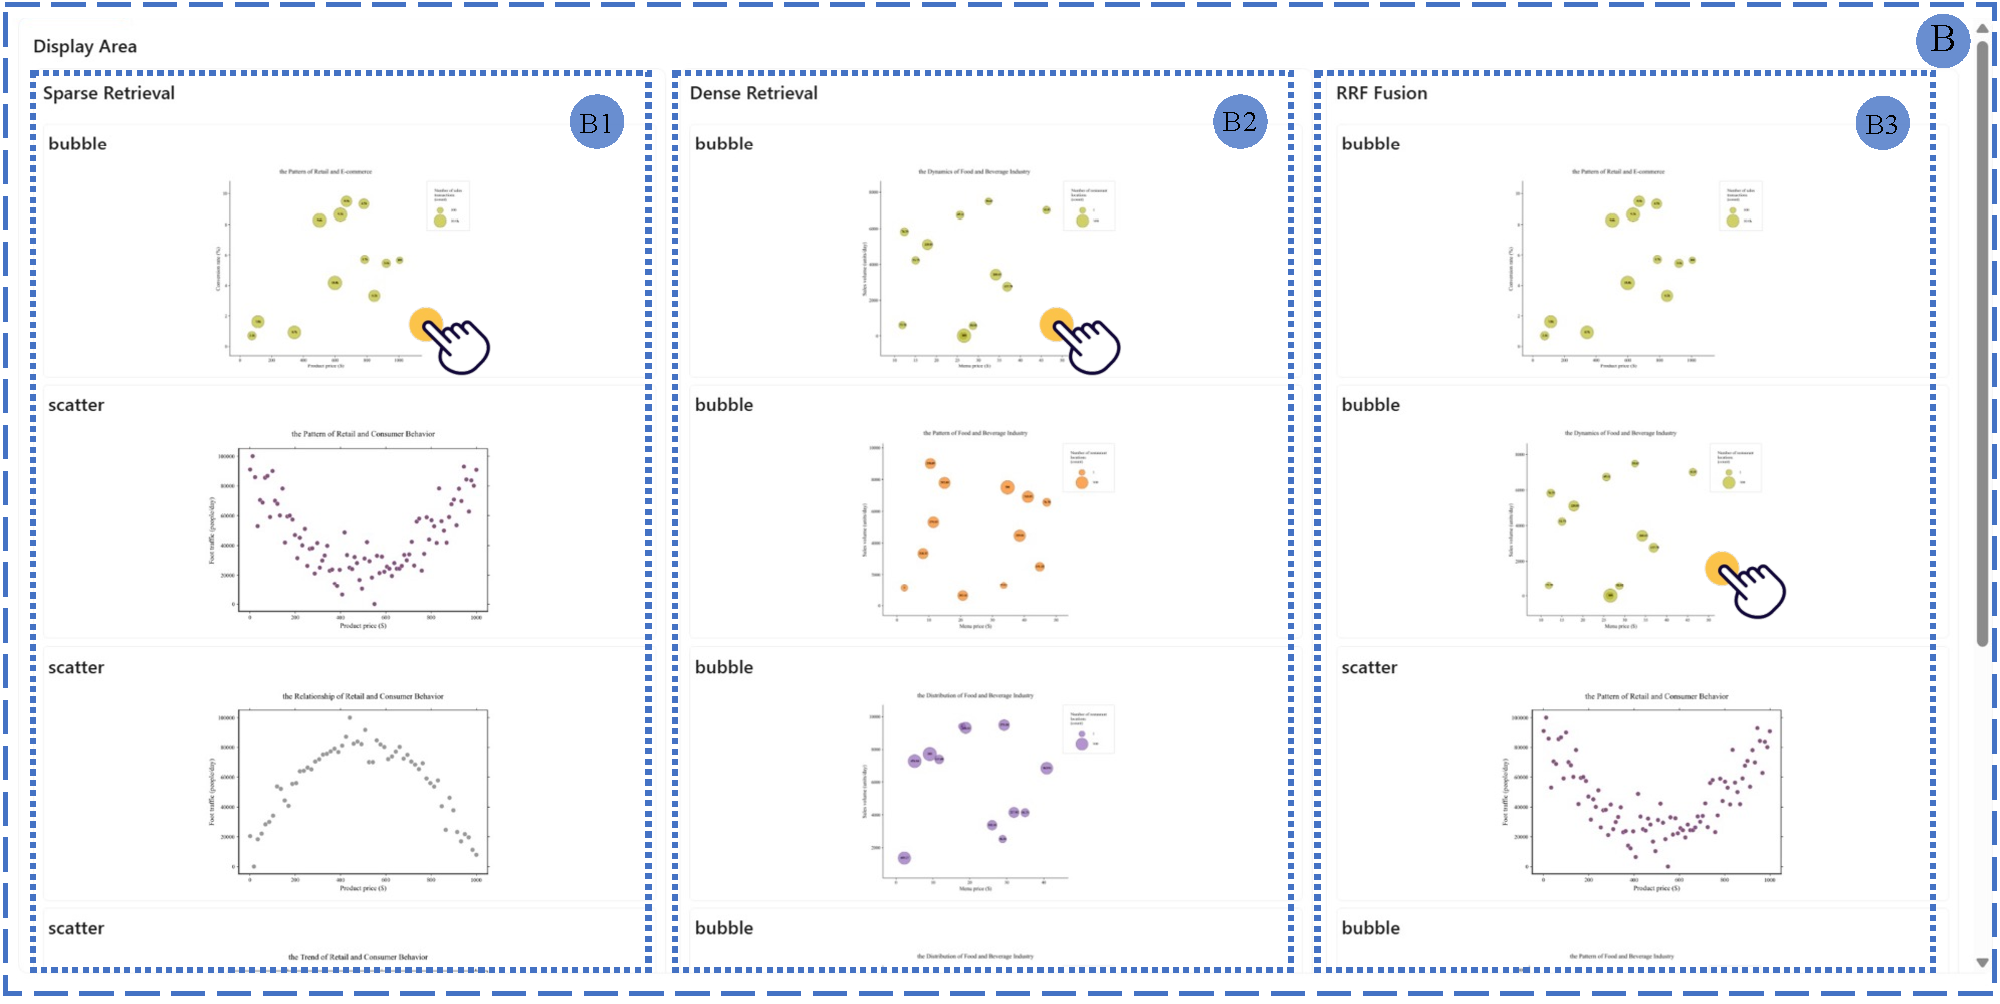
\includegraphics[width=\linewidth]{pics/Display_area.pdf}
    \caption{检索结果展示区}
    \label{fig:placeholder}
\end{figure}

\subsubsection{图表推荐准确性}

推荐系统如图\ref{fig:teaser} 所示。用户首先输入想要可视化的文本（A），然后点击“推荐”按钮。检索结果显示在展示区（B），其中（B1）显示稀疏检索结果，（B2）显示稠密检索结果，（B3）显示通过 RRF 算法融合后的推荐结果。

在步骤2中，用户根据自身需求，分别从（B1）、（B2）和（B3）中选择最合适的图表类型。用户选择的图表类型作为系统推荐反馈，用于进一步评估推荐准确性。在实验中，本文使用 ERR 算法计算推荐准确性。ERR 算法通过衡量用户选择图表与推荐图表之间的匹配情况，并综合考虑推荐序列中的排名信息，为系统提供定量准确性评估。ERR 算法的数学表达如下：

\begin{equation}
    ERR = \sum_{i=1}^{K} \frac{1}{i} R_i\prod_{j=1}^{i-1} (1 - R_j)
\end{equation}

其中，$K$ 表示推荐图表数量，本文取 $K=5$。$i$ 表示当前正在评估的图表位置。$R_i$ 表示第 $i$ 个推荐图表是否与用户选择匹配的指示函数；当 $R_i=1$ 时，表示第 $i$ 个推荐图表与用户选择一致；当 $R_i=0$ 时，表示不一致。$\prod_{j=1}^{i-1}(1-R_j)$ 确保在第 $i$ 个推荐图表之前，所有图表均未与用户选择匹配。

本文计算稀疏检索、稠密检索和 RRF 融合推荐结果的平均相关性、平均贡献度（ERR）以及准确率，如表\ref{tab:err} 所示。从中可以看出，RRF 在相关性、平均贡献度和准确率上均表现优秀，是最能满足用户需求的推荐方法；稠密检索在平均贡献度和准确率上略低于 RRF；稀疏检索在三个方面仍有提升空间。

\begin{table}[htbp]
\centering
\caption{推荐方法评估结果}
\label{tab:err}
\begin{tabular}{cccc}
\toprule
推荐方法 & 平均相关性 & 平均贡献度($Ave_{ERR}$) & 准确率 \\
\midrule
稀疏检索 & 0.78 & 0.62 & 80\% \\
稠密检索 & 0.82 & 0.68 & 85\% \\
RRF & 0.84 & 0.72 & 90\% \\
\bottomrule
\end{tabular}
\end{table}

\subsubsection{用户体验评估}

完成实验步骤3后，本文收集了15名参与者的调查问卷，并对收集到的问卷进行统计，结果如图\ref{fig:userstudy} 所示。问卷采用5分制李克特量表，共包含5个问题。关于推荐准确性（Q1），参与者的主观感受与第6.2.1节中的结论一致，约73\%的参与者认为实验过程中 RRF 推荐结果最符合其需求。参与者认为三种推荐方法给出的结果多样性相近（Q2），这可能也与数据集中图表种类数量有限有关。在推荐图表与输入文本相关性方面，几乎所有参与者都认为 RRF 给出的推荐高度相关（Q3）。在系统可用性和整体满意度方面，大部分参与者给出了正面评价（Q4、Q5）。

\begin{figure}[htbp]
    \centering
    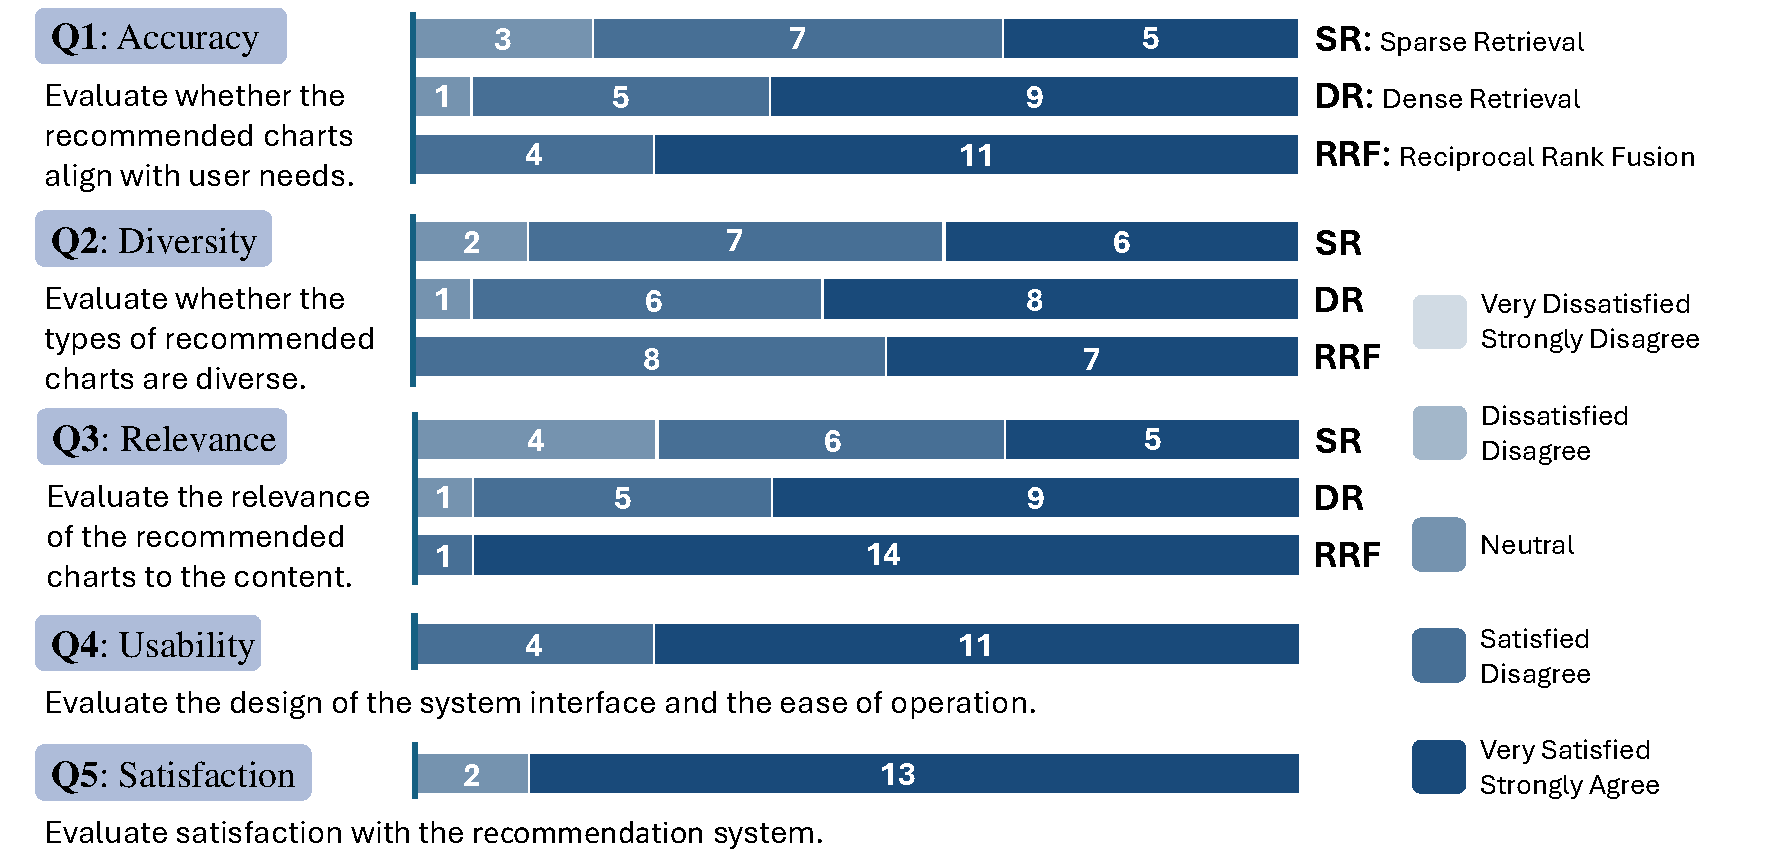
\includegraphics[width=0.8\linewidth]{pics/user_study.pdf}
    \caption{用户研究问卷结果}
    \label{fig:userstudy}
\end{figure}

本文还收集了参与者对推荐系统的开放性反馈，以更好了解其看法和建议。参与者普遍认为该系统使用起来非常方便。用户只需输入文本，系统即可推荐适合体现该文本中数值信息的图表（R1）；三种推荐算法的结果按列排列，也能够帮助数据科学初学者更好理解和解释推荐结果（R2）。参与者喜欢系统编辑区一开始给出初始图表（R5），因为这样不会削弱数据分析的乐趣。他们认为，制图不应完全自动化，因为自动化虽然可以节省体力劳动，但也可能限制创造力。通过算法和系统提供建议，帮助数据分析人员或图表制作者反复迭代和修改（R4），已经能够满足他们的需求和心理预期。

\newpage
